\documentclass[review]{iise}% manuscript submitted for review
%\documentclass{iserc}% final manuscript

\usepackage{multirow}

\conference{Proceedings of the IISE Annual Conference \& Expo 2023 \\
K. Babski-Reeves, B. Eksioglu, D. Hampton, eds.}% Do not change this line.


\title{\titlesize Template and Detailed Paper Guidelines}

\author{
No Author 1 Yet\\No Organization Yet\\No Location Yet \\
\vspace{0.3cm}% Space beween authors with a different affiliation.
No Author 2 Yet\\No Organization Yet\\No Location Yet}
\authorlist{Last Name 1, Last Name 2 and Last Name 3}%Heading
\abstractID{1234}% Fill in the web conference management system-assigned abstract ID.

\begin{document}
\maketitle

\begin{abstract}
{\small For the abstract section heading, use 12-point, Times New Roman, bold, centered font, followed by a single blank line.  Then include the abstract for your paper (max 250 words), using 10-point, Times New Roman, full-justified font.  Include a single blank line after the abstract.}
\end{abstract}


\section*{Keywords}
Industrial engineering, operations research, stochastic processes (Include three to five keywords related to the main topic. This section does not have a section number.)


\section{Page Layout}
All papers are limited to 6 pages (\textit{including title and author data, references, and figures and tables}) and should follow the following format and layout: 
\begin{itemize}
\item Page Size: 8.5" x 11" (Letter)
\item Top and bottom margins: 1.00"
\item Left and right margins: 1.00"
\item First page header: Conference proceedings editors’ information (follow this template)
\item Header (from pages two to six):  No header for initial submission. The last names of the authors will be included in the header for accepted manuscripts during final submission.
\item Spacing and Justification:  Single line-spacing with full-justified text
\item Paragraphs: No indentation of paragraphs. Use a single blank line to separate paragraphs.
\item No footers or page numbers.
\end{itemize}

\section{Paper/Case Study Title}
The following information should be included at the top of the first page: 
\begin{itemize}
\item Paper title:  16-point, Times New Roman, bold, centered, upper and lower case.
\item Abstract ID (initial submission): 12-point, Times New Roman, bold, and centered.
\item Leave space on this page for author names and organizations to ensure the 6-page limit is not exceeded if the manuscript is accepted.
\end{itemize}

\section{Text Sections and Headings}
\subsection{Text Sections and Headings}
Text should be organized into sections and subsections.  A single line should separate paragraphs; no paragraph indentations should be used.  

Font guidelines are as follows:
\begin{itemize}
\item Section Headings: Numbered, 12-point, Times New Roman, bold, upper and lower case, left-justified. Leave one blank line above only.
\item Section Sub-headings: Numbered, 10-point, Times New Roman, bold, upper and lower case, left-justified. Leave one blank line between subsections.
\item Regular text: 10-point, Times New Roman, full-justified, with a single line between paragraphs.
\end{itemize}

\subsection{Bullets}
Bullet guidelines are as follows:
\begin{itemize}
	\item First level bullet.
	\begin{itemize}
		\item Second level bullet
		\begin{itemize}
			\item Third level bullet
		\end{itemize}
	\end{itemize}
\end{itemize}

\section{Figures, Tables and Their Captions}
Tables and figures should be included in the main text (see Figure~\ref{fig1} and Table~\ref{tab1}), as close to the point of their introduction as possible.  Figure and table numbering should be independent.  Captions guidelines are as follows:

\begin{itemize}
\item Table captions: 10-point, Times New Roman, centered (if a single line) or full-justified (if multiple lines). Place caption above the table; leave one blank line above and below the caption.  For an example, see Table~\ref{tab1} below.
\item 10-point, Times New Roman, centered (if a single line) or full-justified (if multiple lines). Place caption below the figure; leave one blank line above and below. As an example, see Figure~\ref{fig1}.
\end{itemize}


\begin{table}[htb]
\caption{Example table for demonstration}\label{tab1}
\vspace{-0.7cm}%Workaround to be conform with the .doc style. Only for table captions.
\begin{center}
\begin{tabular}{ll|ccc}
\hline
\multicolumn{2}{l}{}  & Conservative & Epoch & Improvement (\%)\\ \hline
\multirow{3}{*}{Six epochs} & Federation run time & 1.1 & 0.44 & 62.8\\ \cline{2-5}
 & Number of time advance messages exchanged & 1.1 & 0.44 & 62.8\\ \cline{2-5}
 & Number of checking messages exchanged & 34302 & 23533 & 31.4\\ \cline{2-5}
\end{tabular}
\end{center}
\end{table}

This is an example paragraph to demonstrate the guidelines for figure and table captions.

\begin{figure}[htb]
	\centering
	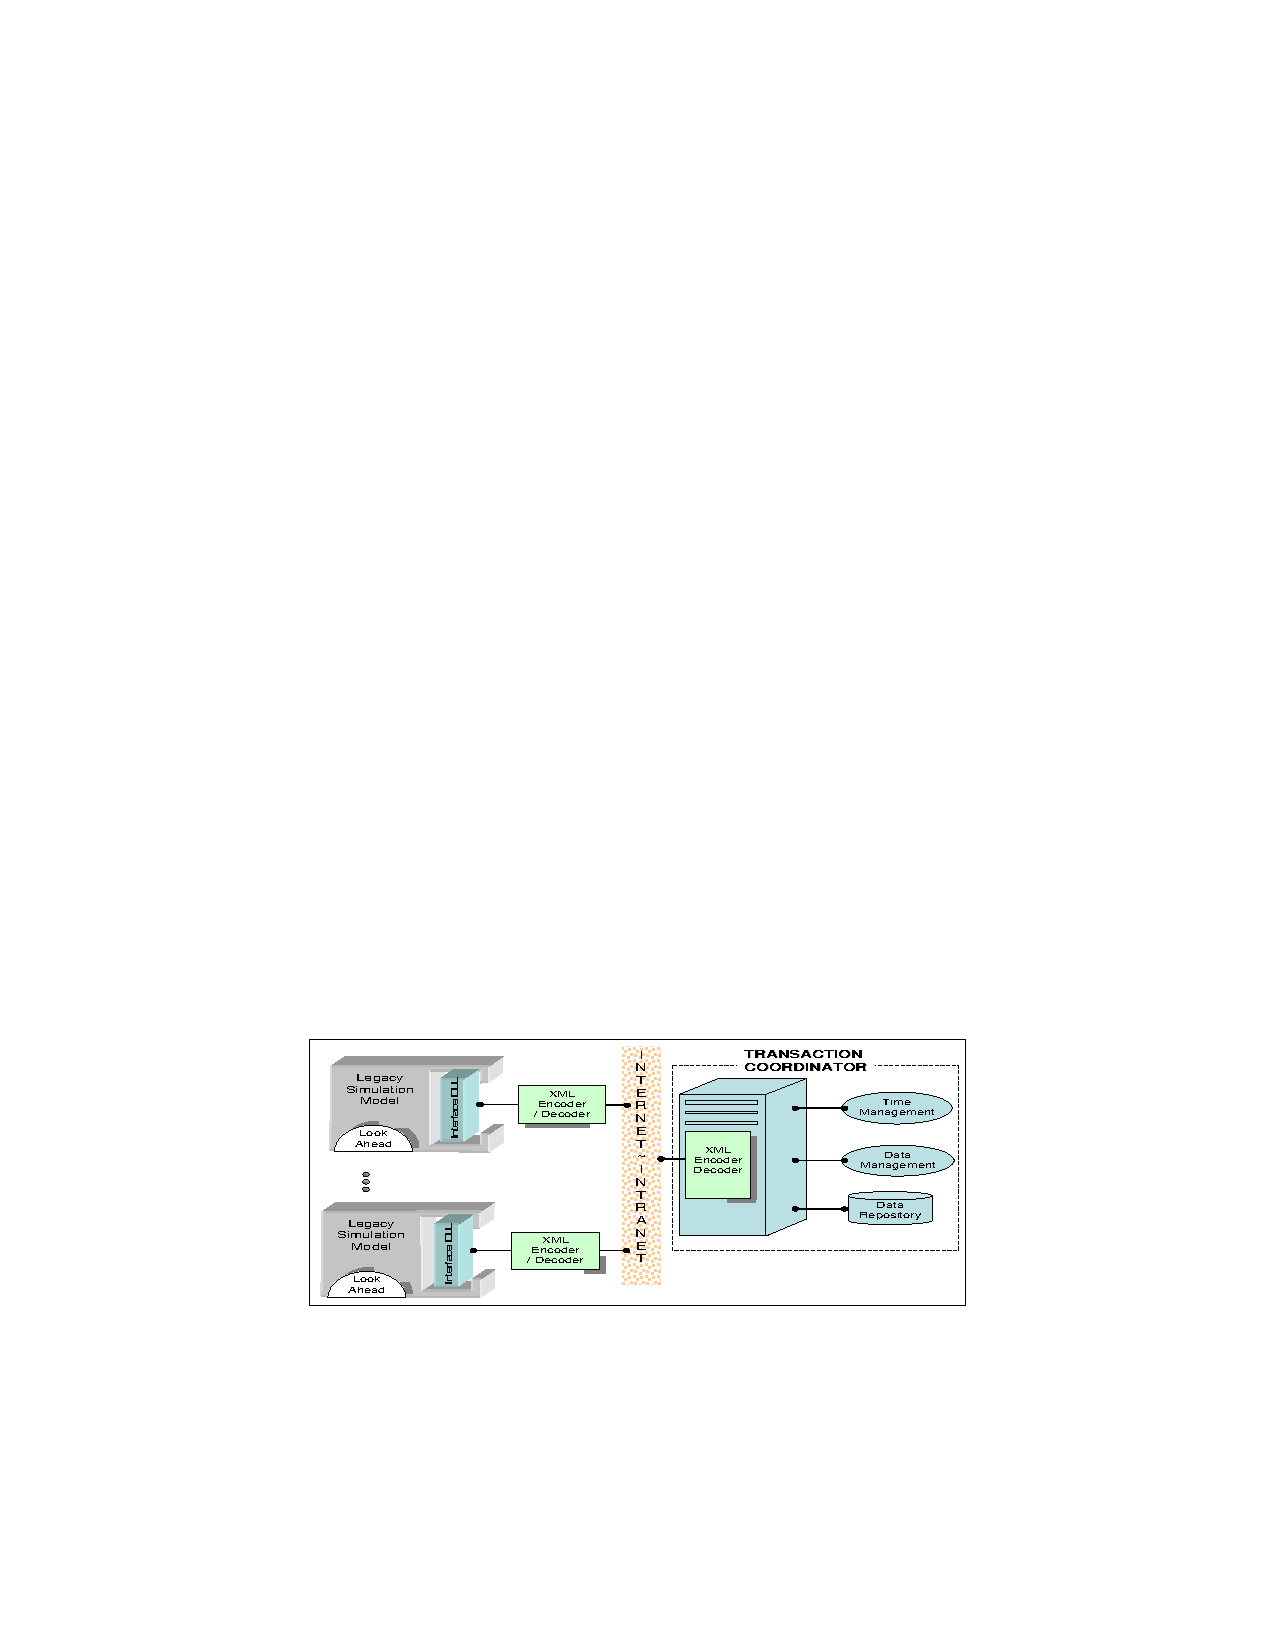
\includegraphics[width=3.5in]{IISE_Figure}
	\caption{Example figure for demonstration}\label{fig1}
\end{figure}


\section{Equations}
Equations should be centered and numbered in order of appearance.  Place the equation number in parentheses, positioned flush to the right margin. Prepare equations with an Equation Writer; screenshots of equations should not be used. Leave one line before and after every equation. See Equation~(\ref{eq1}) below as an example.

\begin{equation}
FD_t = FD_{t-1} + \rho\delta(DIS_t - FD_{t-1})
\label{eq1}
\end{equation}


\section*{Acknowledgements}
Acknowledgement of funding support and/or any other kind of assistance should be contained in an ``Acknowledgements'' section (this section should have no section number), located immediately before the ``References and Citations'' section.

\section*{References and Citations}
The IEEE style should be followed for references and citations for each manuscript submitted to the IISE Annual Conference. In brief, references are numbered sequentially by order of occurrence (not alphabetically) in the text and listed in a separate section labeled References (no section number) at the end of the manuscript. Within the text, they should be cited by the corresponding list number in square brackets \cite{son03}.  When referring to two references, use this format \cite{son06,ven051}.  If you refer to more than two documents listed consecutively, use this format \cite{ven052,ven053,cha06,ush99,raj00}.   The following provides example formats for different types of reference documents.

\begin{thebibliography}{1}

\bibitem{son03}
Son, Y., Wysk, R., and Jones, A., 2003, \newblock ``Simulation Based Shop Floor Control: Formal Model, Model Generation and Control Interface," \newblock
IIE Transactions on Design and Manufacturing, 35(1), 29-48.

\bibitem{son06}
Son, Y., and Venkateswaran, J., 2006, \newblock ``Hierarchical Supply Chain Planning Architecture for Integrated Analysis of Stability and Performance," \newblock
International Journal of Simuation and Process Modeling (in press).

\bibitem{ven051}
Venkateswaran, J., and Son, Y., 2005, Production and Distribution Planning for Dynamic Supply Chains Using Multi-resolution Hybrid Models, Simulation (submitted).

\bibitem{ven052}
Venkateswaran, J., 2005, \newblock ``Production and Distribution Planning for Dynamic Supply Chains Using Multi-resolution Hybrid Models," \newblock
Ph.D. dissertation, The University of Arizona.

\bibitem{ven053}
Venkateswaran, J., and Son, Y., 2005, \newblock ``Information Synchronization Effect on the Stability of Collaborative Supply Chain," \newblock
Proc. of the Winter Simulation Conference, December 4-7, Orlando, Florida, 1668-1676.

\bibitem{cha06}
Chang, T., Wysk, R., and Wang, H., 2006, Computer-Aided Manufacturing, 3rd Edition, Prentice Hall, New Jersey.

\bibitem{ush99}
Usher, J.M., 1999, \newblock ``Chapter 9: STEP Standard in Design and Manufacturing," \newblock
appears in Direct Engineering: Toward Intelligent Manufacturing, Kamrani, A.K. and Sferro, P. (eds.) Kluwer Academic Publishers, Boston, 259-284.

\bibitem{raj00}
Rajgopal, J., and Needy, K.L., 2000, \newblock ``Paper Submission Instructions for IERC 2001," \newblock
(15 August 2000).

\end{thebibliography}


\end{document}
